\section{Controlled User Study}
\label{sec:study}

The purpose of the study is to quantitatively and qualitatively evaluate
the effectiveness of \tool compared to the DAG-based visualizations
found in Gitk or the git command line. The study is broken into three
task-based sections; conceptual tasks, summarization tasks, and
participant opinions. The study was performed during June of 2017
%in Kingston ON,
in a controlled environment running Ubuntu 14.04.
Participants were allowed to use both Gitk and the git command line
tools together, which we will refer to as the git tools or as Gitk. Then
they were asked to perform the same tasks using \tool.

\dmg{I thought you had randomized the order of tool use? also clarify that they were done with different commits to
  avoid bias}

% \evan{Do I need to say where the study took place? I see it showing up
%   in other papers, but it makes it kind of obvious about the lab I'm
%   talking about, doesn't it?}

The primary goal of the study is to determine if \tool is more capable
of providing the participants of our study with a better conceptual
understanding of how a commit is integrated into the kernel, and a
better summarization of various metrics about the files and authors
involved with the integration. The conceptual questions are to determine
if the DAG-based visualizations (gitk and git command line) provide enough information to determine how a
commit, and any related commits, are merged into a project. \tool
displays this information directly in the form of a tree, so we will not
be performing a comparison on this section, only evaluating the results
from Gitk. The summarization tasks compare \tool and Gitk, with the
participants using one tool followed by the other on two commits from
merge-trees of differeing sizes. In both of these sections, the
participant is given a task that they are to find an answer to; we
evaluate the time it took, if the answer was correct, and how far from
the right answer they were. The user opinions provide us with a clear
comparison between the tools from the point-of-view of the participant,
providing us information about which aspects of each tool they prefered.

\subsection{Tasks}
\label{sub:tasks}

% \dmg{use tasks, not questions. you are asking them to do something that requires an answer, that is different than a question}

\dmg{I don't like how you talk about the DAG comprehension. Few paragraphs above I replaced it
  with the DAG-based tools, which might be a better description, since you are evaluating tool
vs tool}

\begin{table*}[htpb]
  \centering
  \caption{Conceptual Tasks }
  \label{tab:conceptual_tasks}
  \begin{tabulary}{0.9\textwidth}{LL}
    \toprule
    Task & Description\\
    \midrule
    T1 & Draw a diagram showing how this commit was merged into the master branch, along with any other related commits\\
    T2 & How many individual commits are related to this commit?\\
    T3 & How many merges are involved with merging this commit into the master branch?\\
    \bottomrule
  \end{tabulary}
\end{table*}

\begin{table}[htpb]
  \centering
  \caption{Summarization Tasks}
  \label{tab:summarization_tasks}
  \begin{tabulary}{\linewidth}{LLL}
    \toprule
    Task Set   & Task & Description\\\midrule
    Merge      & T4   & What is the series of merges involved with merging this
    commit?\\
    & T5   & What other commits are merged?\\
    Authorship & T6   & How many authors are involved?\\
    & T7   & Who contributed the most changes?\\
    Files      & T8   & How many files were modified?\\
    & T9   & Which file had the most changes?\\
    Modules    & T10  & Which modules does this merge tree involve?\\
    \bottomrule
  \end{tabulary}
\end{table}


\textbf{The conceptual tasks} are designed to gain better insight on the
comprehension of the DAG, and determine if the DAG is sufficient for
understanding what other commits are related to a given commit, and how
those commits are merged. The tasks are outlined in
Table~\ref{tab:conceptual_tasks}. The tasks are performed in order
using the git tools. T1 has the participant draw a diagram of the merge
tree, which will be used to answer the other two questions. This enables
us to visually see issues with comprehending the DAG visualizations.
Participants are given 10 minutes to perform this task, which also is
used to familiarize the participant with the git tools interface, if
they are not already, and with the set of commits they will be working
with. T2 and T3 are drawn directly from the diagram from T1, giving
quantitative metrics to measure the comprehension. T2 asks the
participant to verify the number of commits, and T3 asks for the number
of merges. The three tasks are performed on both commits before
continuing to the summarization tasks.


\textbf{The summarization tasks}, listed in Table~\ref{tab:summarization_tasks},
are designed to compare the ability of the participants to summarize
information about the two commits used in the study when using git tools\dmg{be consistent, either you say dag-based
  tools, or git tools, either one is fine, but be consistent}
versus \tool. The tasks are broken into four sets based on what is being
summarized: merges, authorship, files, and modules. The order that the
participants perform each task is randomized within each task set, and
the order of the task sets are then randomized with the exception of the
merges task set which will always come first. We measure and evaluate
three metrics for each task: correctness, accuracy, and timing.
Correctness measures whether the answer was correct or incorrect.
Accuracy measures how far from being correct the provided answer was.
Timing is the duration, in seconds, that the participant took to answer
the task. We begin timing the task at the end of the question, and stop
timing before the last modification to the answer. For this reason, it
is possible for times to overlap between tasks if the participant
changes their answer after answering another question. This will also
modify the answer used for measuring the accuracy. We measure the timing
from the screen capture.

\evan{Is this better, or do you still want me to move the information
  about the randomization to the bottom?}
\dmg{I didn't see anything about choosing what commits to inspect here... but this section looks good}



While the merge task set is part of the summarization task group, it
works less with the summarization of the commits and more with
comprehension of the models. The task is designed with two goals in
mind; first we want to measure and define which commits and which merges
the participant has defined to be in the merge tree; second to help
solidify which commits and merges will be used in the merge tree.

T4 provides a concrete series of merges that the participant believes to
be integrating the commit into the repository. T5 provides a concrete
set of commits that are related to the commit. We place these tasks
first as the answers to these will be necessary for the participant to
answer the tasks that follow, specifically finding the merge into the
master branch. T6 and T7 are related to the authorship at merges,
determining how many authors are involved and who made the most changes.
T8 and T9 are related to the files that were modified in the merge,
determining how many files were modified and which file had the most
changes. T10 is related to the modules that were modified in the merge.
Modules are not explicitly defined in git, but are a property of the
Linux repository that we noticed while looking at various commits. To
find the modules, take the text up to the first colon in the git log
preview. For the log preview \textit{``ALSA: kernel docs: fix
  sound/core/ kernel-doc''} the module is \textit{``ALSA''}, e.g.

The accuracy metrics are measured slightly differently between tasks due
to different requirements and structures in the answer. In task T4, both
the order and the merges are important. We define the distance to be the
edit distance with insertion, deletion, and transposition at unit cost.
The accuracy is the minimum edit distance necessary to make the answer
correct. T5, T9, and T10 are concerned with the set of elements in the
response; the order is not important. We use the Levenshtein distance,
with insertion, deletion, and substitution operations of unit cost, from
the provided answer to the correct answer. The answers to T6 and T8 are
single number values; the distance is measured as the absolute value of
the difference between the provided answer and the correct answer. T7
has only a single correct answer, thus the distance would either be zero
or one. For this reason, it is acceptable to omit the accuracy metric
from this task. The correctness metric is simply whether the answer was
correct or not; an accuracy of zero indicates a correct answer.

Statistical significance testing is performed to verify that the results
are meaningful. We use $alpha = 0.05$ or a $95\%$ confidence level. The
McNemar $\chi^2$ test\cite{McNemar1947} with continuity correct is used
to test the statistical significance of the hypothesis that \tool
improves correctness of the participants. The $\chi^2$ threshold
statistic at $\alpha = 0.05$ is 3.841. The Wilcoxon\cite{Wilcoxon45}
test and Cliff's effect size\cite{Cliff93} are applied to the accuracy
and timing metrics to determine the significance of the difference
between \tool and Gitk. The Wilcoxon test is applied between commits to
determine if the size of the merge-tree effects timing and accuracy. The
null hypotheses and alternative hypotheses are stated in
Table~\ref{tab:null_alt_hypoths}.

\begin{table*}[h!]
  \centering
  \caption{Null and Alternative Hypotheses for Summarization Tasks\evan{Should I say exactly
      what the null hypotheses are referring to (counting authors,
      files, etc... or is this good enough? It's already a huge and
      redundant table) }}
  \label{tab:null_alt_hypoths}
  \begin{tabulary}{0.98\linewidth}{CCLL}
    \toprule
    Task & Metric             & Null Hypothesis                                                      & Alternative Hypothesis\\\midrule
    T4   & \tiny{Commit}      & There is no difference on accuracy or timing between \comA and \comB & There is a difference on accuracy or timing between \comA and \comB \\
    T4   & \tiny{Correctness} & \tool does not effect the correctness of the participants            & \tool does effect the correctness of the participants\\
    T4   & \tiny{Accuracy}    & There is no difference between \tool and Gitk on accuracy            & There is a difference between \tool and Gitk on accuracy\\
    T4   & \tiny{Timing}      & There is no difference between \tool and Gitk on timing              & There is a difference between \tool and Gitk on timing\\

    T5   & \tiny{Commit}      & There is no difference on accuracy or timing between \comA and \comB & There is a difference on accuracy or timing between \comA and \comB \\
    T5   & \tiny{Correctness} & \tool does not effect the correctness of the participants            & \tool does effect the correctness of the participants\\
    T5   & \tiny{Accuracy}    & There is no difference between \tool and Gitk on accuracy            & There is a difference between \tool and Gitk on accuracy\\
    T5   & \tiny{Timing}      & There is no difference between \tool and Gitk on timing              & There is a difference between \tool and Gitk on timing\\

    T6   & \tiny{Commit}      & There is no difference on accuracy or timing between \comA and \comB & There is a difference on accuracy or timing between \comA and \comB \\
    T6   & \tiny{Correctness} & \tool does not effect the correctness of the participants            & \tool does effect the correctness of the participants\\
    T6   & \tiny{Accuracy}    & There is no difference between \tool and Gitk on accuracy            & There is a difference between \tool and Gitk on accuracy\\
    T6   & \tiny{Timing}      & There is no difference between \tool and Gitk on timing              & There is a difference between \tool and Gitk on timing\\

    T7   & \tiny{Commit}      & There is no difference on accuracy or timing between \comA and \comB & There is a difference on accuracy or timing between \comA and \comB \\
    T7   & \tiny{Correctness} & \tool does not effect the correctness of the participants            & \tool does effect the correctness of the participants\\
    T7   & \tiny{Accuracy}    & There is no difference between \tool and Gitk on accuracy            & There is a difference between \tool and Gitk on accuracy\\
    T7   & \tiny{Timing}      & There is no difference between \tool and Gitk on timing              & There is a difference between \tool and Gitk on timing\\

    T8   & \tiny{Commit}      & There is no difference on accuracy or timing between \comA and \comB & There is a difference on accuracy or timing between \comA and \comB \\
    T8   & \tiny{Correctness} & \tool does not effect the correctness of the participants            & \tool does effect the correctness of the participants\\
    T8   & \tiny{Accuracy}    & There is no difference between \tool and Gitk on accuracy            & There is a difference between \tool and Gitk on accuracy\\
    T8   & \tiny{Timing}      & There is no difference between \tool and Gitk on timing              & There is a difference between \tool and Gitk on timing\\

    T9   & \tiny{Commit}      & There is no difference on accuracy or timing between \comA and \comB & There is a difference on accuracy or timing between \comA and \comB \\
    T9   & \tiny{Correctness} & \tool does not effect the correctness of the participants            & \tool does effect the correctness of the participants\\
    T9   & \tiny{Accuracy}    & There is no difference between \tool and Gitk on accuracy            & There is a difference between \tool and Gitk on accuracy\\
    T9   & \tiny{Timing}      & There is no difference between \tool and Gitk on timing              & There is a difference between \tool and Gitk on timing\\

    T10   & \tiny{Commit}      & There is no difference on accuracy or timing between \comA and \comB & There is a difference on accuracy or timing between \comA and \comB \\
    T10   & \tiny{Correctness} & \tool does not effect the correctness of the participants            & \tool does effect the correctness of the participants\\
    T10   & \tiny{Accuracy}    & There is no difference between \tool and Gitk on accuracy            & There is a difference between \tool and Gitk on accuracy\\
    T10   & \tiny{Timing}      & There is no difference between \tool and Gitk on timing              & There is a difference between \tool and Gitk on timing\\
    \bottomrule
  \end{tabulary}
\end{table*}


\textbf{The user-opinion} questions, listed in
Table~\ref{tab:opinion_questions}, are designed to determine which tool
provides a better user experience for summarization and comprehension
tasks, and what aspects of each assisted with their understanding. T11
asks for the preference of the participant, given that their goal is
comprehension and summarization. % TODO add T11 results
We recognize that neither tool is perfect, and participants may have
complaints about both tools, but are interested in what parts of each
tool assisted them with understanding the events in the repository. T12
is meant to address this. % TODO add T12 results


\begin{table}[htpb]
  \centering
  \caption{User-Opinion Questions}
  \label{tab:opinion_questions}
  \begin{tabulary}{0.9\linewidth}{LL}
    \toprule
    Task & Description\\
    \midrule
    T11 & Given these tasks again, which tool would you prefer?\\
    T12 & Which aspects of each tool did you like and why?\\
    \bottomrule
  \end{tabulary}
\end{table}


\subsection{Commit Selection}
\label{sub:commit_selection}

We include two commits in the study to detect differences between merge
tree sizes. The order that the commits are presented to each participant
is randomized. We analyzed the 15096 merge-trees from April 16th 2005 to
October 14th 2014, which corresponds to the releases Linux 2.6.12-rc3
and Linux 3.17-rc1. 25\% of the trees contain at most a single commit
not including the root, while 50\% of the trees contain at most seven
nodes non-root nodes. 75\% of the trees contain at least 51 nodes, and
the largest tree contains 7217 nodes.

From this information, we selected one tree with a single commit, and
one tree with seven other nodes to represent a small tree and a
medium-sized tree. A majority of the trees are flat, where all nodes
merge directly into the root node. Of the 8031 trees containing at least
seven nodes, only 593 contained at least a single internal merge node.
Trivially, trees with a single node cannot have any internal nodes, and
of the 624 trees with seven nodes, only 135 contained at least one inner
node. To increase the complexity of the medium-sized tree, we randomly
selected one of the 135 trees to represent the medium tree.

From the 2008 trees containing only a single node, we selected one at
random, and trivially selected the only commit in the tree. From the
trees containing seven nodes, we selected one randomly, then randomly
selected one of the commits in the tree. We selected commit
\emph{a3c1239eb59c0a907f8be5587d42e950f44543f8} from the tree containing
a single node, which we will refer to as \comA, and commit
\emph{cdbdd1676a5379f1d5cbd4d476f5e349f445befe} from the tree containing
seven nodes, which we will refer to as \comB. A visual representation
for these trees is shown in Figure~\ref{fig:study_commits}.

\begin{figure}[bpt]
  \centering
  \begin{tabular}{ m{1.5cm} m{3cm} }
    
\includegraphics[height=0.5in]{figures/commits/1-commit.pdf} &
    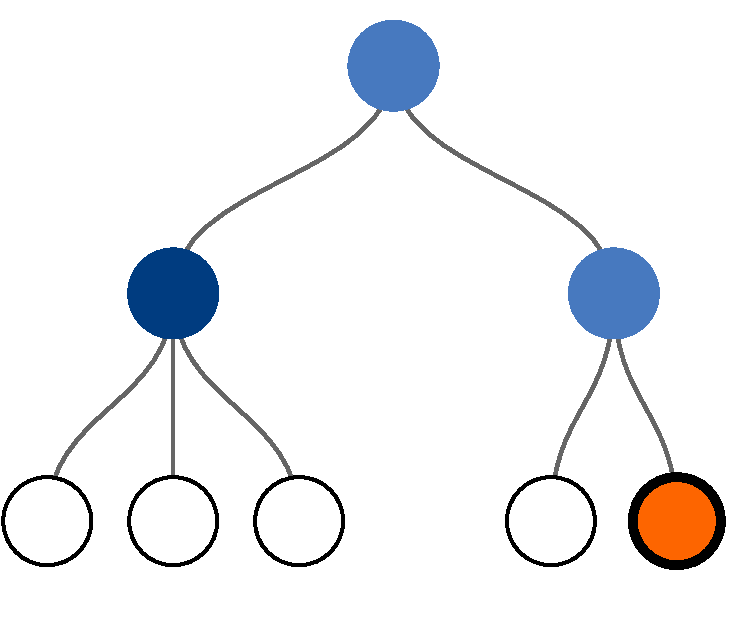
\includegraphics[height=1in]{figures/commits/7-commits.pdf}\\
  \end{tabular}
  \caption{The merge trees used in the user study,
    containing one and seven commits, respectively.}
  \label{fig:study_commits}
\end{figure}

\subsection{Participant Profile}
\label{sub:participant_profile}

The study was conducted with 12 participants, all of whom were
masters, PhD, or post-doc researchers in the field of software
engineering. The participants had between 6 months and 10 years
experience with git, with the median being 3.5 years. Most of the
participants had additional experience with SVN and CVS.\@ One of the
participants in the study worked as a release engineer, studying merge
practices to determine the best way to merge branches while minimizing
the number of merge conflicts, on SVN repositories. The participants
worked with repositories ranging from around 10 commits up to 38000
commits, with the median being 350 commits. Two of the participants had
never collaborated with anyone in a repository, while the rest had some
experience with repositories being modified by multiple people, with the
most being 219. The median number of collaborators was four.

Five participants had only worked with personal and academic
repositories. Two participants had worked with school and
professional repositories, and two had only worked with professional
repositories. One participant worked with personal, academic, and
professional repositories, one participant had only worked with personal
repositories, and one participant had worked with personal, academic,
and school repositories.
\dmg{you made it confusing: just say: how many had experience with
  professional repositories and remove the above
}
\evan{Do you want more information about the participants?}

All participants have had at least some experience with the idea of
version control, branching in repositories, and git. The participants
are all from the same lab, and each participant worked with both tools
in the study, thus, keeping the sample populations identical for both
tools, with some variation between participants in experience with
repositories.

\dmg{BIG QUESTION}
for each task, did they do always git tools then linvis for the same commit?  if so, there is potential for learning
bias: they learn the structure of the commits with git tools, so therefore it was easier for them to do
them with linvis.
\dmg{END QUESTION}

\dmg{I'll stop here today}


\subsection{Study Procedure}
\label{sub:study_procedure}

The study begins with a short introduction to the \mt model, followed by
an introduction to Gitk and \tool. We provided two examples of
converting the DAG to the \mt. The first DAG was a flat merge, so the
corresponding merge tree did not have any internal nodes. The second was
not a flat merge, so the corresponding merge tree contained a single
internal node. Any questions about the model were answered at this time.
Following the introduction to the \mt model, we introduce Gitk and
\tool, providing information about what each pane shows in Gitk, and
what each tab does in \tool.

The conceptual tasks follow the introduction, followed by the
summarization, which are then followed by the user opinion. The study is
completed with three questions to enable us to know more about the
participants;

\begin{itemize}
  \item How long have you used git?
  \item For what kind of projects have you used git?
  \item How many commits, files, and collaborators were involved with
    the largest repository you have worked with?
\end{itemize}



To mitigate the order bias cased by using one tool before the other or
one commit before the other, we randomize both the tool and commit
between participants. The conceptual tasks are run twice, once with
\comA and once with \comB, in the same order for all participants using
the git tools.

\evan{This paragraph is kind of tricky to explain well. See if you can
  understand what I'm trying to say} The summarization tasks are run
four times, once with \comA and \tool, \comB and \tool, \comA and git
tools, and \comB and git tools. The participant will start with one
tool, and complete the tasks for both commits in that tool. The order of
the commits is the same as in the conceptual tasks. Once they complete
the summarization tasks for both \comA and \comB, they will switch to
the other tool and complete the tasks again on the commits in the same
order. The order of the tasks is consistent for all four runs.

The user opinions do not directly involve working with the tools or the
commits, so the ordering of the tools

% To mitigate the order bias caused by using one tool before the other,
% one commit before the other, and the various tasks, we randomize...

We use a script written in python 3.6.1 in order to assure that we do no
bias the randomization, and ensure that correct ordering is maintained
between tools, tasks, and commits. The script produces the entire script
for the study, so we only need to read it to correctly conduct the
study. Re-running the script generates the study for the next
participant. We use screen capture to record the audio and video. From
the screen capture, we measure the time, as well as recording the
responses in the study.

\evan{Should I include the python script? It would make explaining how
  the test was conducted 100\% clear.}

% TODO: maybe move the time measuring procedure from summ. to here

\subsection{Results}
\label{sec:results}

\evan{This looks weird not having text between the subsections... Should
  I put something here?...}

\subsubsection{Conceptual Tasks}
\label{sub:conceptual_tasks}

Table~\ref{tab:conceptual_results} shows a summary of the results from
conceptual tasks T2 and T3. The answer column contains the correct
answer to the corresponding task, while the median, mean, and variance
columns are with respect to the answers provided by the
participants.\evan{Is this better for describing the columns in the
  table?} The median(s), mean(s), and variance(s) columns are with
respect to the time taken, in seconds, by the participants to respond to
the tasks.


\evan{Should I add some of the drawings to the paper?}
The results from T1 did not vary greatly between the participants. The
drawings generally show something in the form of a list, starting from
the provided commit and traversing the master branch, indicating that
the participants were unable to determine which merge was in the master
branch. Many of the participants identified the next tag, v2.6.29-rc6,
to be ``the master branch'', however, a tag is not a branch. One
participant was able to draw the correct diagram for \comA directly
using the git command line, but rejected their response after inspecting
the DAG visualization provided by Gitk and proceeded to draw a list of
merges.


\begin{table*}[htpb]
  \centering
  \caption{Results from the conceptual questions}
  \label{tab:conceptual_results}
  \begin{tabular}{ll|r|lrr|rrr}
    Question & Commit & Answer & Median & Mean  & Variance & Median(s) & Mean(s) & Variance(s)\\\hline\hline
    T2       & \comA  & 1      & 4      & 19.11 & 753.11   & 10.0      & 49.92   & 5952.08\\
    T3       & \comA  & 1      & 5      & 8.27  & 53.62    & 7.5       & 24.67   & 884.42\\\hline
    T2       & \comB  & 5      & 4      & 7.80  & 136.84   & 31.5      & 106.83  & 54123.42\\
    T3       & \comB  & 3      & 3.5    & 5.40  & 50.27    & 11.0      & 65.6    & 29798.82\\
  \end{tabular}
\end{table*}

Users were able to more closely estimate the number of commits and
merges in the larger tree, but generally took longer than the smaller
tree. The tree with a single node resulted in more variability in the
estimate of number of commits.

It should be noted that these questions were answered after spending
roughly ten minutes attempting to draw a picture that held the answers
to these questions, so the times indicate how quickly the participant
was able to interpret their conceptual understanding.

\subsubsection{Summarization Tasks}
\label{sub:summarization_tasks}

Table~\ref{tab:cross_commit_results} shows whether the merge-tree size
has an effect on the three studied metrics. An interesting observation
from the figure is that the corrected for T5 and T9 are effected by the
size of the merge-tree, but the accuracy is not. The correctness results
for T5 and T9 are shown in Figure~\ref{fig:correctness_t5_t9}, and the
timing results for T7 are shown in Figure~\ref{fig:timing_t7}.

\begin{table}[htpb]
  \centering
  \caption{Cross-Commit Results\evan{Should I group the results by task
      or by metric? It's by metric right now}}
  \label{tab:cross_commit_results}
  \begin{tabular}{ccrl}
    \toprule
    Task & Metric      & $p$-value & Conclusion\\\midrule
    T4   & Correctness & 0.22      & Do not reject $H_0$\\
    T5   & Correctness & 0.04      & Reject $H_0$\\
    T6   & Correctness & 0.13      & Do not reject $H_0$\\
    T7   & Correctness & 0.06      & Do not reject $H_0$\\
    T8   & Correctness & 0.07      & Do not reject $H_0$\\
    T9   & Correctness & 0.04      & Reject $H_0$\\
    T10  & Correctness & 0.62      & Do not reject $H_0$\\

    T4  & Accuracy & 0.94 & Do not reject $H_0$\\
    T5  & Accuracy & 0.09 & Do not reject $H_0$\\
    T6  & Accuracy & 0.19 & Do not reject $H_0$\\
    T8  & Accuracy & 0.16 & Do not reject $H_0$\\
    T9  & Accuracy & 0.08 & Do not reject $H_0$\\
    T10 & Accuracy & 0.37 & Do not reject $H_0$\\

    T4  & Time & 0.77 & Do not reject $H_0$\\
    T5  & Time & 0.97 & Do not reject $H_0$\\
    T6  & Time & 0.90 & Do not reject $H_0$\\
    T7  & Time & 0.01 & Reject $H_0$\\
    T8  & Time & 0.87 & Do not reject $H_0$\\
    T9  & Time & 0.99 & Do not reject $H_0$\\
    T10 & Time & 0.68 & Do not reject $H_0$\\
    \bottomrule
  \end{tabular}
\end{table}

\begin{figure*}[htpb]
  \centering
  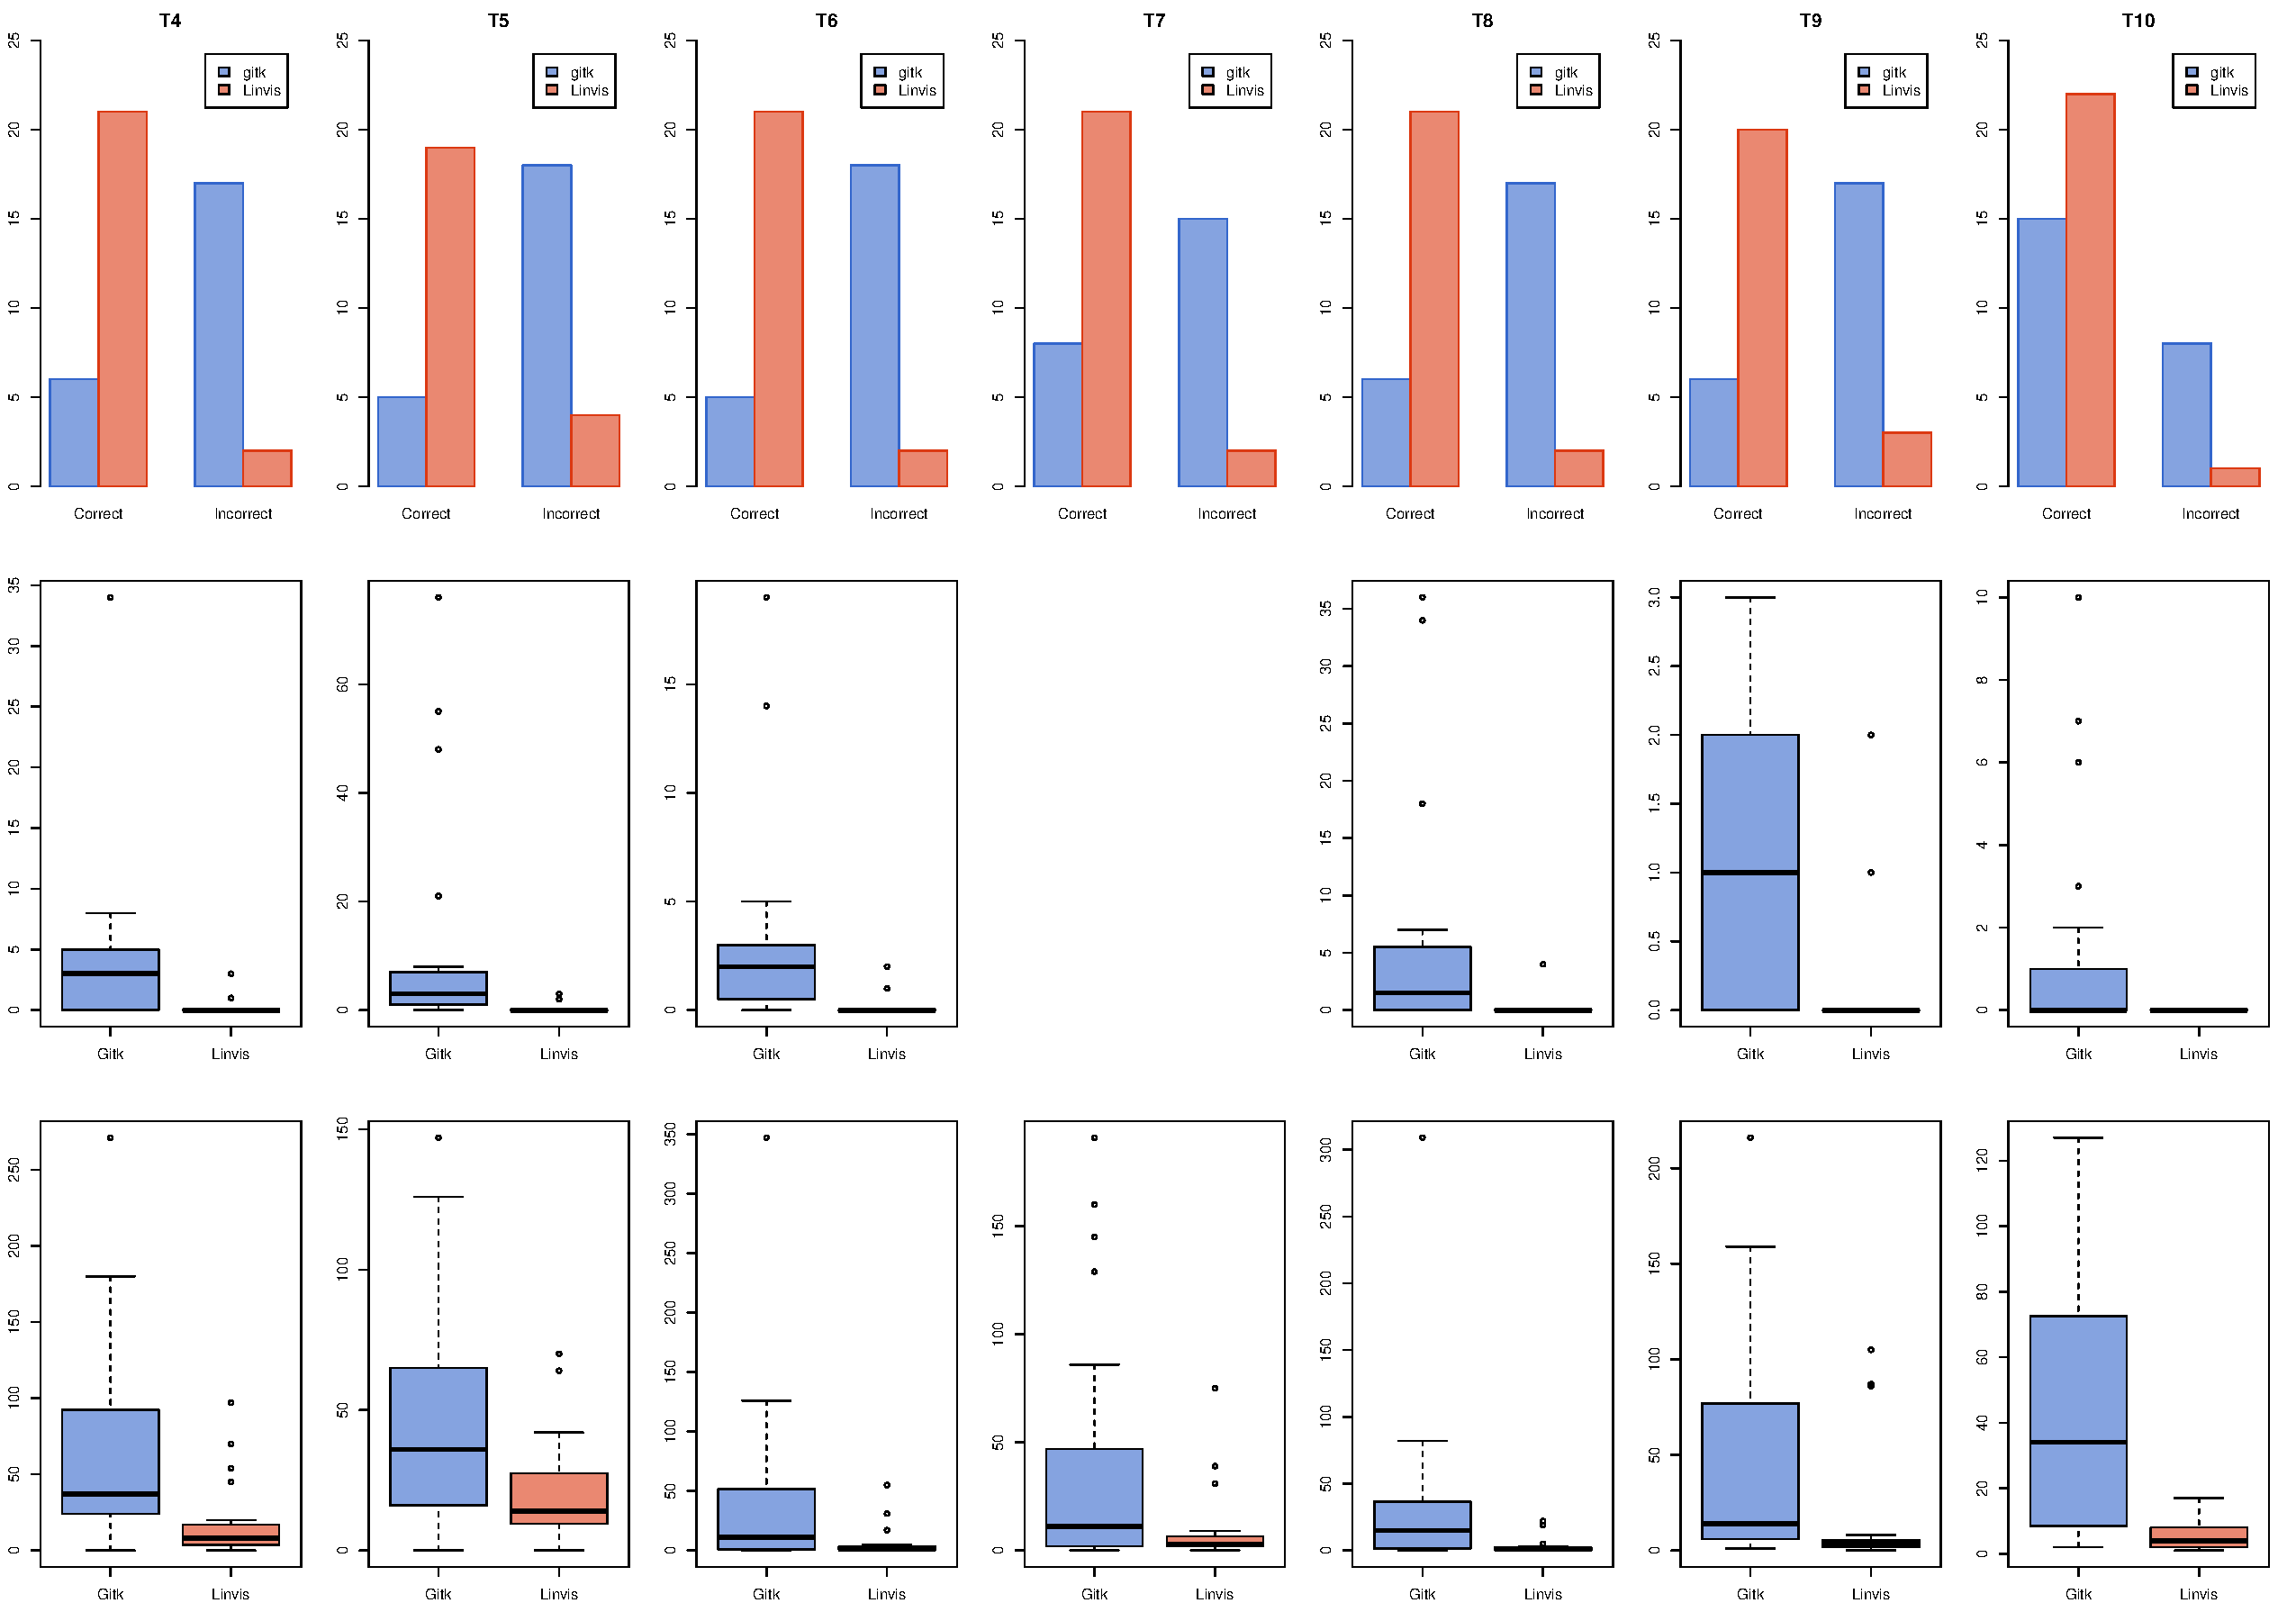
\includegraphics[width=\textwidth]{figures/userstudy/results.pdf}
  \caption{Aggregated results from the summarization tasks. The first row plots the
    correctness metric for each task. The second row plots the
    accuracy metric for each task. The third row plots the time metric
    for each task. The correctness results for T5, T9, and the timing
    results for T7 cannot be aggregated across commits, thus are
    omitted.}
  \label{fig:summarization_results}
\end{figure*}

\begin{figure*}[htpb]
  \centering

  \begin{tabular}{ m{6cm} m{6cm} }
    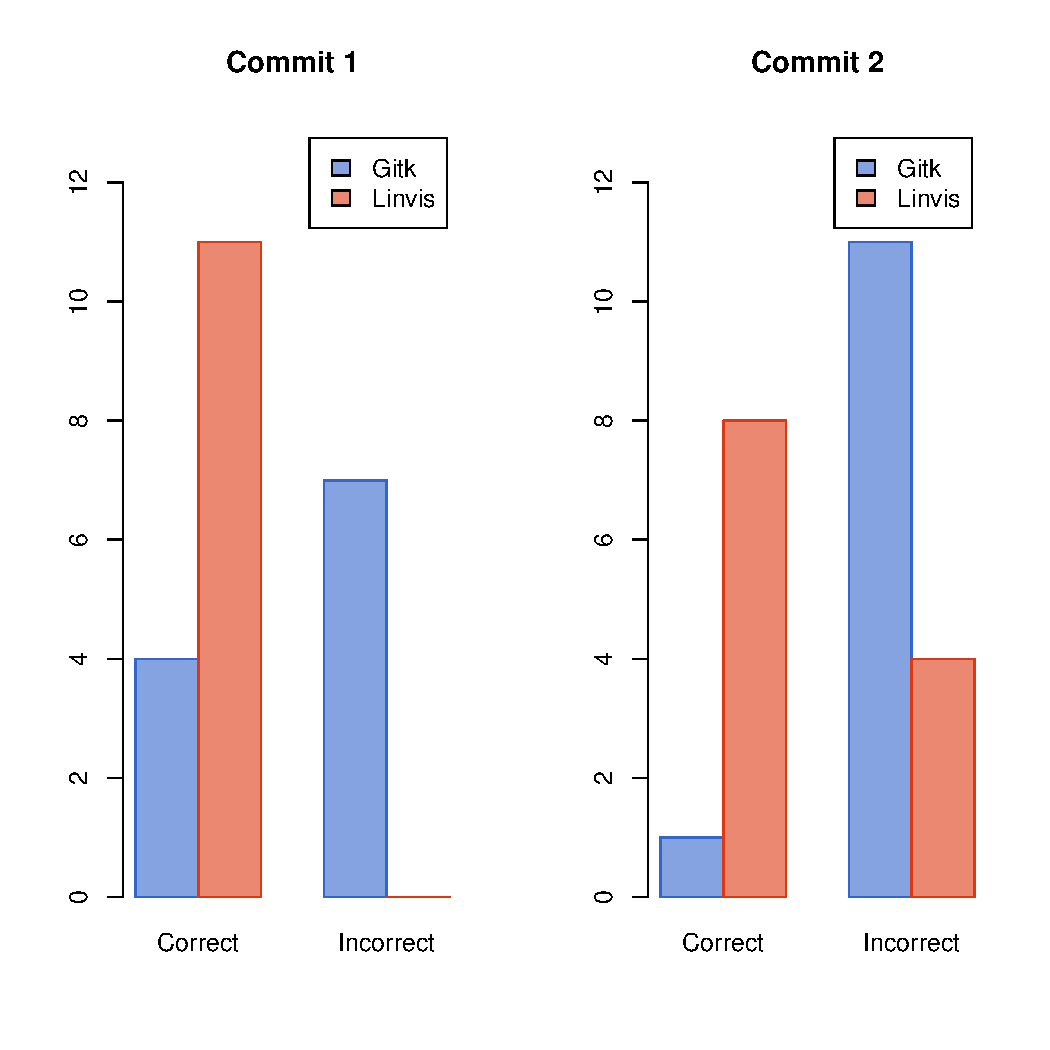
\includegraphics[width=6cm]{figures/userstudy/correctness/5.pdf} &
    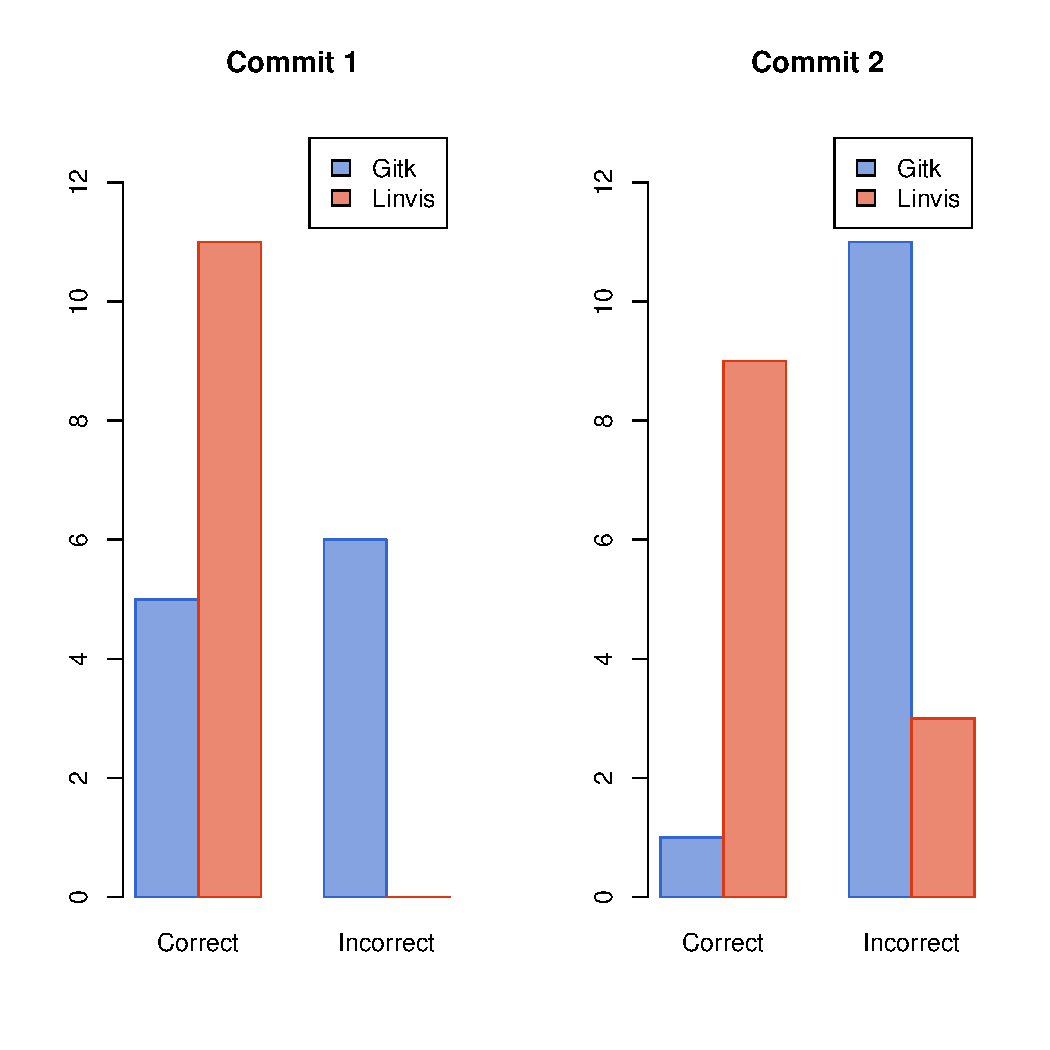
\includegraphics[width=6cm]{figures/userstudy/correctness/9.pdf}
  \end{tabular}
  \caption{Unaggregated Correctness results for T5 and T9 \evan{Split
      this? Is it clear that between Commit 2 and Commit 1 is where the
    separation of the plots is?}}
  \label{fig:correctness_t5_t9}
\end{figure*}

\begin{figure}[htpb]
  \centering
  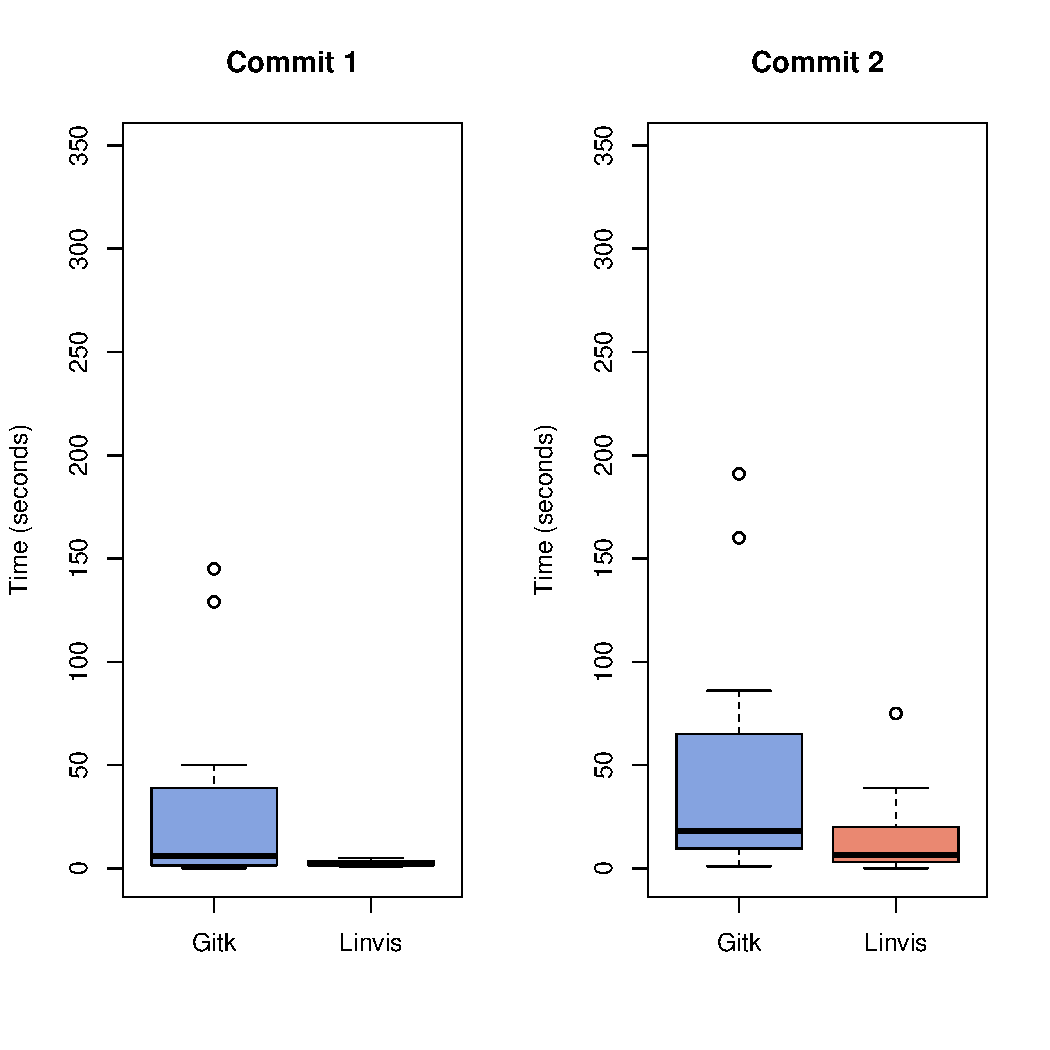
\includegraphics[width=0.8\linewidth]{figures/userstudy/time/7.pdf}
  \caption{Unaggregated Timing results for T7}
  \label{fig:timing_t7}
\end{figure}

\begin{table*}[htpb]
  \centering
  \caption{Summarized Correctness, Accuracy, and Timing results for the summarization tasks}
  \label{tab:summarization_table}
  \begin{tabular}{ccc}
    % Correctness
    \begin{tabular}{crrc}
      \toprule
      Task                  & $\chi^2$ & $p$-value  & Conclusion\\\midrule
      T4                    & 13.07    & 0.0003     & Reject $H_0$\\
      \multirow{2}{*}{T5}   & 5.14     & 0.0233     & Reject $H_0$\\
                            & 5.14     & 0.0233     & Reject $H_0$\\
      T6                    & 14.06    & 0.0002     & Reject $H_0$\\
      T7                    & 11.07    & 0.0009     & Reject $H_0$\\
      T8                    & 13.07    & 0.0003     & Reject $H_0$\\
      \multirow{2}{*}{T9}   & 4.17     & 0.0412     & Reject $H_0$\\
                            & 6.13     & 0.0133     & Reject $H_0$\\
      T10                   & 4.00     & 0.0455     & Reject $H_0$\\
      \bottomrule
    \end{tabular}
    &

    % Accuracy
    \begin{tabular}{clrc}
      \toprule
      Task & $p$-value            & Delta Est. & Conclusion\\\midrule
      T4   & $7.8 \times 10^{-5}$ & -0.61      & Reject $H_0$\\
      T5   & $7.2 \times 10^{-5}$ & -0.63      & Reject $H_0$\\
      T6   & $1.2 \times 10^{-5}$ & -0.69      & Reject $H_0$\\
      T8   & $5.8 \times 10^{-4}$ & -0.54      & Reject $H_0$\\
      T9   & $0.009$              & -0.42      & Reject $H_0$\\
      T10  & $0.002$              & -0.35      & Reject $H_0$\\
      \bottomrule
    \end{tabular}
    &
    % Timing
    \begin{tabular}{clrc}
      \toprule
      Task                 & $p$-value & Delta Est. & Conclusion\\\midrule
      T4                   & 0.0007    & -0.58      & Reject $H_0$\\
      T5                   & 0.0142    & -0.42      & Reject $H_0$\\
      T6                   & 0.0168    & -0.41      & Reject $H_0$\\
      \multirow{2}{*}{T7}  & 0.2586    & -0.29      & Do not reject $H_0$\\
                           & 0.0780    & -0.43      & Do not reject $H_0$\\
      T8                   & 0.0009    & -0.57      & Reject $H_0$\\
      T9                   & 0.0002    & -0.63      & Reject $H_0$\\
      T10                  & 0.0001    & -0.66      & Reject $H_0$\\
      \bottomrule
    \end{tabular}
  \end{tabular}
\end{table*}

Summaries for correctness, accuracy, and timing are shown in
tables~\ref{tab:summarization_table}.
The full results are as follows;

\begin{itemize}
  \item T4

    \textbf{Correctness:}
    The $\chi^2$ statistic is $13.07$ with a p-value of $0.0003$.
    $13.07 > 3.841$ and $0.0003 < 0.05$, therefore we reject the null
    hypothesis.
    \vspace{2mm}
    \begin{tabular}{cc|rr}
                            &           & \multicolumn{2}{c}{Linvis}\\
                            &           & Correct                      & Incorrect\\\hline
      \multirow{2}{*}{Gitk} & Correct   & 6                            & 0\\
                            & Incorrect & 15                           & 2\\
    \end{tabular}
    \vspace{3mm}

    \tool improves the correctness when determine the series of merges
    involved with merging a commit.

    \textbf{Accuracy:} The p-value is $7.8 \times 10^{-5}$, which is
    less than 0.05; therefore we reject the null hypothesis. The Delta
    estimate is -0.61, which indicates a large effect size. \tool
    improves accuracy when determining the series of merges involved
    with merging a commit.

    \textbf{Timing:}
    The p-value is $0.0007$, which is less than 0.05; therefore we
    reject the null hypothesis. The delta estimate is -0.58, which
    indicates a large effect size. \tool decreases the time taken to
    determine the series of merges involved with merging a commit.

    Overall, \tool is able to help users determine the series of merges
    that a commit takes more quickly and more accurately than Gitk.

  \item T5

    \textbf{Correctness:}
    The correctness results are split for this task. For \comA, the
    $\chi^2$ statistic is $5.14$ with a $p-value$ of $0.02334$. $5.14 >
    3.841$ and $0.02334 < 0.05$, therefore we reject the null
    hypothesis.
    \vspace{2mm}
    \begin{tabular}{cc|rr}
                             &           & \multicolumn{2}{c}{Linvis}\\
                             &           & Correct                      & Incorrect\\\hline
      \multirow{2}{*}{Gitk}  & Correct   & 4                            & 0\\
                             & Incorrect & 7                            & 0\\
    \end{tabular}
    \vspace{3mm}

    The $\chi^2$ statistic for \comB is $5.14$ with a p-value of
    $0.02334$. $4.14 > 3.841$ and $0.02334 < 0.05$, therefore we reject
    the null hypothesis.
    \vspace{2mm}
    \begin{tabular}{cc|rr}
                             &           & \multicolumn{2}{c}{Linvis}\\
                             &           & Correct                      & Incorrect\\\hline
      \multirow{2}{*}{Gitk}  & Correct   & 1                            & 0\\
                             & Incorrect & 7                            & 4\\
    \end{tabular}
    \vspace{3mm}

    While there is a difference in correctness between different-sized
    merge-trees, \tool improves correctness of determining the other
    commits related to a commit in trees of varying sizes.

    \textbf{Accuracy:}
    The p-value is $7.2 \times 10^{-5}$, which is less than 0.05;
    therefore we reject the null hypothesis. The Delta estimate is
    -0.63, which indicates a large effect size. \tool improves
    accuracy when determining other commits related to a commit.


    \textbf{Timing:}
    The p-value is $0.0142$, which is less than 0.05; therefore we
    reject the null hypothesis. The delta estimate is -0.58, which
    indicates a large effect size. \tool decreases the time taken to
    determine other commits related to a commit.

    Overall, \tool helps users determine other commits that are merged
    with another commit more quickly and more accurately.

  \item T6

    \textbf{Correctness:}
    The $\chi^2$ statistic is $14.06$ with a p-value of $0.0002$.
    $14.06 > 3.841$ and $0.0002 < 0.05$, therefore we reject the null
    hypothesis.
    \vspace{2mm}
    \begin{tabular}{cc|rr}
      &           & \multicolumn{2}{c}{Linvis}\\
      &           & Correct                      & Incorrect\\\hline
      \multirow{2}{*}{Gitk} & Correct   & 5                            & 0\\
      & Incorrect & 16                           & 2\\
    \end{tabular}
    \vspace{3mm}

    \tool improves correctness when determining how many authors are
    involved with a merge.

    \textbf{Accuracy:} The p-value is $1.2 \times 10^{-5}$, which is
    less than 0.05; we reject the null hypothesis. The delta estimate is
    -0.69, which indicates a large effect size. \tool improves accuracy
    when determining how many authors are involved with a merge.

    \textbf{Timing:} The p-value is 0.0168, which is less that 0.05; we
    reject the null hypothesis. The delta estimate is -0.41, which
    indicates a medium effect size. \tool decreases the time taken to
    determine the number of authors involved in a commit.

    Overall, \tool assists users with determining the number of authors
    involved in a merge more quickly and more accurately.

  \item T7

    \textbf{Correctness:}
    The $\chi^2$ statistic is $11.07$ with a p-value of $0.0009$.
    $11.07 > 3.841$ and $0.0009 < 0.05$, therefore we reject the null
    hypothesis.
    \vspace{2mm}
    \begin{tabular}{cc|rr}
      &           & \multicolumn{2}{c}{Linvis}\\
      &           & Correct                      & Incorrect\\\hline
      \multirow{2}{*}{Gitk} & Correct   & 8                            & 0\\
      & Incorrect & 13                           & 2\\
    \end{tabular}\\
    \vspace{3mm}

    \tool improves the correctness of participants when determining the
    author that contributed the most changes to a merge.

    \textbf{Timing:} The null hypothesis is not rejected in the case of
    \comA, but is rejected in the case of \comB. This indicates that
    \tool is able to help users determine who made the most
    contributions to a merge in a large tree than in a small tree.

    Overall, \tool improves the correctness for trees of various sizes,
    but only has an effect on the amount of time taken when the tree is
    large.

  \item T8

    \textbf{Correctness:}
    The $\chi^2$ statistic is $13.07$ with a p-value of $0.0003$.
    $13.07 > 3.841$ and $0.0003 < 0.05$, therefore we reject the null
    hypothesis.
    \vspace{2mm}
    \begin{tabular}{cc|rr}
      &           & \multicolumn{2}{c}{Linvis}\\
      &           & Correct                      & Incorrect\\\hline
      \multirow{2}{*}{Gitk} & Correct   & 6                            & 0\\
      & Incorrect & 15                           & 2\\
    \end{tabular}\\
    \vspace{3mm}

    \textbf{Accuracy:} The p-value is $5.8 \times 10^{-4}$, which is
    less than 0.05; we reject the null hypothesis. The delta estimate is
    -0.54, indicating a large effect size. \tool improves accuracy when
    determining how many files were modified at a merge.

    \textbf{Timing:} The p-value is 0.0009, which is less than 0.05; we
    reject the null hypothesis. The delta estimate is -0.57, indicating
    a large effect size.

  \item T9

    \textbf{Correctness:}
    The correctness results are split for this task. For \comA, the
    $\chi^2$ statistic is $4.17$ with a p-value of $0.0412$. $4.17 >
    3.841$ and $0.0412 < 0.05$, therefore we reject the null hypothesis.
    \vspace{2mm}
    \begin{tabular}{cc|rr}
                             &           & \multicolumn{2}{c}{Linvis}\\
                             &           & Correct                      & Incorrect\\\hline
      \multirow{2}{*}{Gitk}  & Correct   & 5                            & 0\\
                             & Incorrect & 6                            & 0\\
    \end{tabular}
    \vspace{3mm}

    The $\chi^2$ statistic for \comB is $6.125$ with a p-value of
    $0.0133$. $6.125 > 3.841$ and $0.0133 < 0.05$, therefore we reject
    the null hypothesis.
    \vspace{2mm}
    \begin{tabular}{cc|rr}
                             &           & \multicolumn{2}{c}{Linvis}\\
                             &           & Correct                      & Incorrect\\\hline
      \multirow{2}{*}{Gitk}  & Correct   & 1                            & 0\\
                             & Incorrect & 8                            & 3\\
    \end{tabular}
    \vspace{3mm}

    \textbf{Accuracy:} The p-value is $0.009$, which is less than
    $0.05$; we reject the null hypothesis. The delta estimate is -0.42,
    indicating a medium effect size. \tool improves accuracy when
    determining which file had the most changes.

    \textbf{Timing:} We reject the null hypothesis; the delta estimate
    is -0.63, indicating a large effect size. \tool decreases the time
    taken to determine which file had the most changes.

    Overall, \tool is able to assist users determine which file had the
    most changes more quickly and accurately.

  \item T10

    \textbf{Correctness:}
    The $\chi^2$ statistic is $4$ with a p-value of $0.0455$.
    $4 > 3.841$ and $0.0455 < 0.05$, therefore we reject the null
    hypothesis. The p-value is very close to the $\alpha$ value in this
    case, so the conclusion is not as well defined.
    \vspace{2mm}
    \begin{tabular}{cc|rr}
      &           & \multicolumn{2}{c}{Linvis}\\
      &           & Correct                      & Incorrect\\\hline
      \multirow{2}{*}{Gitk}   & Correct   & 14                           & 1\\
      & Incorrect & 8                            & 0\\
    \end{tabular}
    \vspace{3mm}

    \textbf{Accuracy:} The null hypothesis is rejected; the delta
    estimate is -0.35, indicating a medium effect size. \tool provides
    an improvement in accuracy when determining which modules are
    involved with a merge.

    \textbf{Timing:} The null hypothesis is rejected; the delta estimate
    is -0.66, indicating a large effect size. \tool decreases the time
    taken to determine the modules involved with a merge.

    Overall, \tool assists users determine which modules are involved
    with a merge more quickly and accurately.

\end{itemize}

\tool is able to assist users with summarizing various aspects of a
merge more quickly and accurately than Gitk. In two tasks, T5 and T9,
correctness was affected by the size of a tree, but in both trees, \tool
was able to provide a statistically significant improvement to the
correctness. Only in one task, T7, was timing affected by the size of a
tree; \tool did not significantly improve the time taken to answer T7 on
the smaller tree, but did improve the time taken on the larger tree.

\subsubsection{User Opinions}
\label{sub:user_opinions}

Among the 12 participants, there was nearly unanimous agreement that
for conceptual understanding and summarization tasks, \tool was easier
to work with than Gitk. The participants cited the ability to abstract
information about the merge from the clean summarization tables and
simple visualizations. Three participants suggested that someone with a
professional understanding of Gitk and the git command-line may be to
extract a conceptual understanding from the DAG and perform the
summarization tasks. One of these three participants said that they
would prefer to have both tools available, as they are able to
complement each other.

%%% Local Variables:
%%% mode: latex
%%% TeX-master: "lineval.tex"
%%% End:
